\documentclass[]{article}
% ATLAS macros
\usepackage{atlasphysics}
% Nice maths macros
\usepackage{amsmath}
% Feynman diagrams
\usepackage{feynmp}
% Figures and floats
\usepackage{graphicx,subfig}

% Graphics folider
\graphicspath{{figures/}}

% Read .1 file extension as .mps.
\DeclareGraphicsRule{.1}{mps}{*}{}

\begin{document}

\title{The $\ee \rarrow \mumu$ Cross Section in the Standard Model}
\author{Alex Pearce}
\date{\today}
\maketitle


\begin{abstract}
The Standard Model's (SM) prediction of particles beyond those initially considered by quantum electrodynamics (QED) has yielded excellent results. The Super Proton Synchrotron (SPS) at CERN recently detected both the $\Wboson$ bosons and the $\Zzero$ boson via the $\antibar{p}$ channel (Rubbia, van der Meer et al.). We performed a numerical integration of the differential cross section of the $\ee \rarrow \mumu$ scattering process, which may produce $\Zzero$ bosons, in the hope that the proposed Large Electron-Positron collider (LEP) will verify this channel of $\Zzero$ production. A distinct $\Zzero$ resonance around the $\Zzero$ mass of 91.8\GeV was found with a cross section $\sigma=9.4\inb$.
\end{abstract}


%\tableofcontents


\section{Introduction}\label{sec:intro}

The proposition of three mediators of the weak nuclear force, the $\Wplus$, $\Wminus$ and $\Zzero$ bosons, has been all but proven by the current team at CERN operating the SPS. The suggestion of $\Zzero$ production via electron-positron pairs is now becoming of interest to experimentalists. The process is manifested by an electron-position pair ($e^{-}e^{+}$) annihilating, forming either a virtual photon or $\Zzero$ boson, and then a muon-antimuon pair ($\mu^{-}\mu^{+}$) being produced.

This interaction is described by the Feynman diagram in figure \ref{fig:feynsgammaz}. The scattering is also described by a t-channel diagram (in figure \ref{fig:feyntgammaz}), however we proceed by analysing the s-channel as it is only this channel via which we may measure resonances and new unstable particles. Note that a u-channel diagram also exists, but as it is simply a swapping of the outgoing particles' momenta in the t-channel, hence we ignore this also.

The use of Feynman diagrams is that we may apply the Feynman rules to them to produce a  matrix element $\mathcal{M}$. The square of this corresponds to a differential cross section $\frac{\d{\sigma}}{\d{\Omega}}$ which may be integrated to find the total cross section $\sigma$, which is measurable by a detector.

The following section briefly outlines the theory behind the interactions. The integration methods used to evaluate the differential cross sections are explored in the section after that, along with a study of the differential cross sections in order to judge the effectiveness of numerical integration upon them. The results are presented and analysed in section \ref{sec:results}, then a discussion of the kinematic variables follows in section \ref{sec:variables}. Finally, a brief discussion on performance and alternative numerical integration techniques occurs in section \ref{sec:performance}.

\section{Principles of Interaction Cross Sections}

With reference to the Feynman diagrams in figures \ref{fig:feynsgammaz} and \ref{fig:feyntgammaz}, the incoming particles are labelled with the four-momenta $p_{1}^{\nu}$ and $p_{2}^{\nu}$, whilst the outgoing particles carry $p_{3}^{\nu}$ and $p_{4}^{\nu}$. At LEP, the electrons and positrons (antiparticles to the electron) will be accelerated around a loop in opposite directions. The collider energy is then given $\sqrt{s}$, where $$s = (p_{1} + p_{2})^{2}.$$ Here we have suppressed the metric tensor and covariant notation, implicitly assuming four vectors. The collider energy is then analogous to the hypotenuse of a right-angled triangle of sides $p_{1}^{\nu}$ and $p_{2}^{\nu}$.

The differential cross sections are dependant on the collider energy via the dimensionless variables $$\varepsilon = \frac{m_{\mu}}{\sqrt{s}}, \quad \lambda = \frac{M_{\Zzero}}{\sqrt{s}},$$

where $m_{\mu}$ is the muon mass. It is worth noting that, at the energies LEP will be operating at, it is safe to consider the electron as massless in the ultrarelativistic limit. (In addition, the muon is over 200 times more massive than the electron so we may disregard the electron mass in scattering interactions.)

\subsection{Real and Virtual Particles}

As noted in figure \ref{fig:feynsgammaz}, the scattering may be mediated by either a virtual photon $\gamma^{*}$ or a $\Zzero^{(*)}$ boson, where the bracketed star notation indicates that the boson may either be \emph{on-} or \emph{off-mass-shell}. These terms refer to how well the mediating particles (propagators in the Feynman diagrams) adhere to the mass-energy relation $E^{2} - \lvert{\vec{p}}\rvert^{2}c^{2} = m^{2}c^{4}$. Propagators exceeding the classical relativistic values of $E$ and $p$ are off-shell, and said to be virtual particles. This violation of relativity is allowed because it is permitted by the Heisenberg uncertainty principle, $\Delta E\Delta t \geq \hbar$: the violation in energy may only exist for a very small amount of time.

The $\Zzero$ boson will be on-shell (i.e. real) if and only if $s = M_{\Zzero}$, where $M_{\Zzero}$ is the boson's mass. When the particle is real, we can detect it. With this, we should expect a cross section resonance as the boson tends towards being on-mass.

\subsection{Differential Cross Sections}

The total matrix element $\mathcal{M}$ must be considered carefully. As the propagator in the interaction may be one of two particles, it must be the sum of two separate matrix elements (one matrix element for each possible propagator). The measurable quantity, the cross section, is the integrated square of the matrix element, so we must have the square of a sum:

\begin{align*}
\mathcal{M} &= \mathcal{M}_{\gamma} + \mathcal{M}_{\Zzero},
\\
\mathcal{M}^{2} &= (\mathcal{M}_{\gamma} + \mathcal{M}_{\Zzero})^{2}
\\
&= \mathcal{M}_{\gamma}^{2} + \mathcal{M}_{\Zzero}^{2} + 2\operatorname{Re}(\mathcal{M}_{\gamma}\mathcal{M}_{\Zzero}^{*})
\\
&= \frac{\d{\sigma}}{\d{\Omega}}^{\gamma\operatorname{-}\gamma} +
	\frac{\d{\sigma}}{\d{\Omega}}^{\Zzero\operatorname{-}\Zzero} +
	\frac{\d{\sigma}}{\d{\Omega}}^{\gamma\operatorname{-}\Zzero}
\\
&= \frac{\d{\sigma}}{\d{\Omega}}.
\end{align*}

Each term of $\mathcal{M}^{2}$ corresponds to its own differential cross section: the first for the pure photon process, the second for the pure $\Zzero$ process, and the last for the interference of both processes.

The functional form of each differential cross section is derived by applying the Feynman rules to figure \ref{fig:feynsgammaz}. Due to their bulk, they are not reproduced here but are given in appendix \ref{app:differentials}.


\section{Integration of the Differential $\frac{\d{\sigma}}{\d{\Omega}}$}\label{sec:integration}

A common analytical approach to numerically approximating integrals in the trapezium rule. We use the trapezium rule and compare it with the much more recent Monte Carlo method, whereby random points are sampled and the fraction of those between the curve and the independent axis is proportional to the area i.e. the integral.

The reasoning behind using two methods of numerical integration is twofold. Firstly, it serves as a useful consistency check: if at least one method is running incorrectly, the results from each are unlikely to agree with each other. Secondly, the data collected with respect to the efficiency of each method on the given functions may be useful for future analysis of particle interaction cross sections (or, indeed, any functions of a similar form).

On this point, it is worth noting that the accuracy of each algorithm will depend largely on the functional form of the differential cross sections. Erratic, non-analytic functions will be poorly suited for trapezium evaluation, while functions with very small variations will result in the poor Monte Carlo accuracy. The differential forms are plotted in figures \ref{fig:diffbelow}, \ref{fig:diffexact} and \ref{fig:diffabove}. The impact of these forms in the accuracy of the final results will be analysed in section \ref{sec:results}.

\subsection{Method}\label{ssec:method}

As the integration is over circular polar coordinates, we note that the differential $\sin{\theta}\d{\theta}\d{\phi}$ may be expressed as $\d{(\cos{\theta})}\d{\phi}$, hence we may perform the change of variable $\cos{\theta} \to x$. This changes the limits in $\theta$ to the limits in $x$ $$0 \leq \theta \leq \pi \to -1 \leq x \leq 1.$$ Consequently, the random numbers generated for the Monte Carlo integration are generated between -1 and 1, providing a uniform distribution in $\cos{\theta}$, rather than $\theta$.

A simple Monte Carlo integration will be performed via $$\int\limits_{a}^{b}f(x)\d{x} \approx \frac{b-a}{N}\sum\limits_{i=1}^{N}f(x_{i}),$$ where $N$ is the number of random points to be sampled and $x_{i}$ is the $i^{\mathrm{th}}$ random number with the integration limits.

A similarly simple trapezium algorithm is used: $$\int\limits_{a}^{b}f(x)\d{x} \approx \frac{h(f(a) + f(b))}{2} + h\sum\limits_{i=1}^{N-1}f(a+ih).$$

$h$ is the trapezoidal width, $h=\frac{b-a}{N}$, and $N$ is the number of trapezoids used to estimate the integral with.

Both methods are quoted as approximations, but it should be considered that as $N \to \infty$ the Monte Carlo method becomes exact (despite this being impossible to perform computationally).

The number of points to sample or the number of trapezoids to use will depend on the computation power and time available, as well as the accuracy and precision desired. The exact values used will be discussed in the following section.

\section{Results and Analysis}\label{sec:results}

\TeX


\section{Kinematic Variables}\label{sec:variables}

Discussion of $\cos{\theta}$ and $p_{T} = \lvert\vec{p}_{f}\rvert\sin{\theta}$.


\section{Performance}\label{sec:performance}

TODO Extension of the problem.

\subsection{Runge-Kutta}\label{ssect:rugkut}

Here we are.


\section{Figures}

\subsection{Feynman Diagrams}

\begin{figure}[h]
	\vspace{10pt}
	% Diagram unit length.
	\unitlength = 1mm
	\centering
	\subfloat[s-channel]{
		\label{fig:feynsgammaz}
		\begin{fmffile}{sgammazcrossing}
		  \begin{fmfgraph*}(40,25)
		    \fmfleft{i1,i2}
		    \fmfright{o1,o2}
		    \fmflabel{$e^-$}{i1}
		    \fmflabel{$e^+$}{i2}
		    \fmflabel{$\mu^+$}{o1}
		    \fmflabel{$\mu^-$}{o2}
		    \fmf{fermion}{i1,v1,i2}
		    \fmf{fermion}{o1,v2,o2}
		    \fmf{photon,label=$\gamma^{*}/\Zzero^{(*)}$}{v1,v2}
		  \end{fmfgraph*}
		\end{fmffile}
	}
	\qquad
	\subfloat[t-channel]{
		\label{fig:feyntgammaz}
		\begin{fmffile}{tgammazcrossing}
		  \begin{fmfgraph*}(40,25)
		    \fmfleft{i1,i2}
		    \fmfright{o1,o2}
		    \fmflabel{$e^-$}{i1}
		    \fmflabel{$e^+$}{i2}
		    \fmflabel{$\mu^-$}{o1}
		    \fmflabel{$\mu^+$}{o2}
		    \fmf{fermion}{i1,v1,o1}
		    \fmf{fermion}{o2,v2,i2}
		    \fmf{photon,label=$\gamma^{*}/\Zzero^{(*)}$}{v1,v2}
		  \end{fmfgraph*}
		\end{fmffile}
	}
	\caption{$e^{-}e^{+}\rarrow\mu^{-}\mu^{+}$ scattering via two different channels.}
\end{figure}

\subsection{Differential Cross Sections}

This subsection contains plottings of the QED differential cross section ($\gamma\operatorname{-}\gamma$ channel) and then the full Standard Model cross section ($\gamma\operatorname{-}\gamma$, $\Zzero\operatorname{-}\Zzero$ and $\gamma\operatorname{-}\Zzero$ channels) at three different collider energies.

\begin{figure}[h]
	\vspace{10pt}
	\centering
	\subfloat[QED]{
		\label{fig:diffqedbelow}
		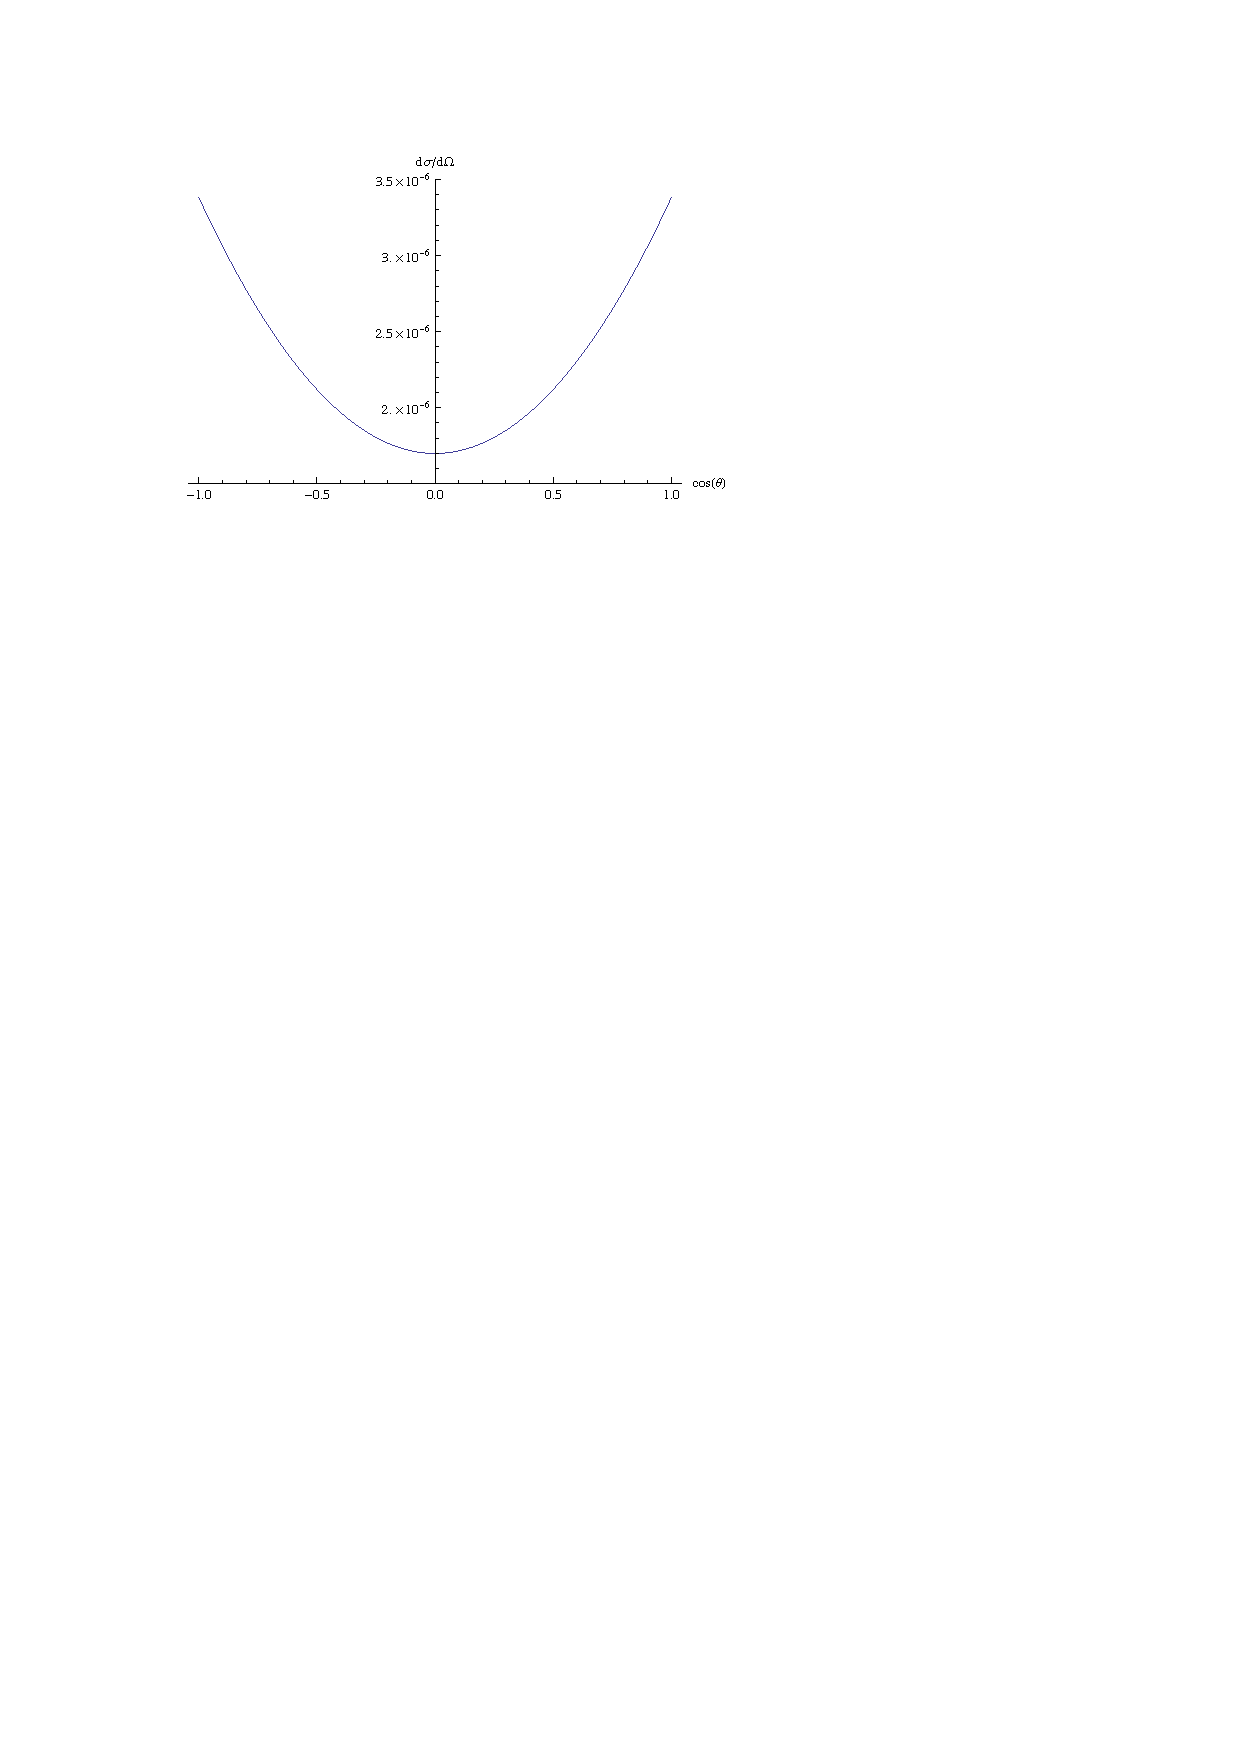
\includegraphics[scale=0.7]{qed_below}
	}
	\subfloat[SM]{
		\label{fig:diffsmbelow}
		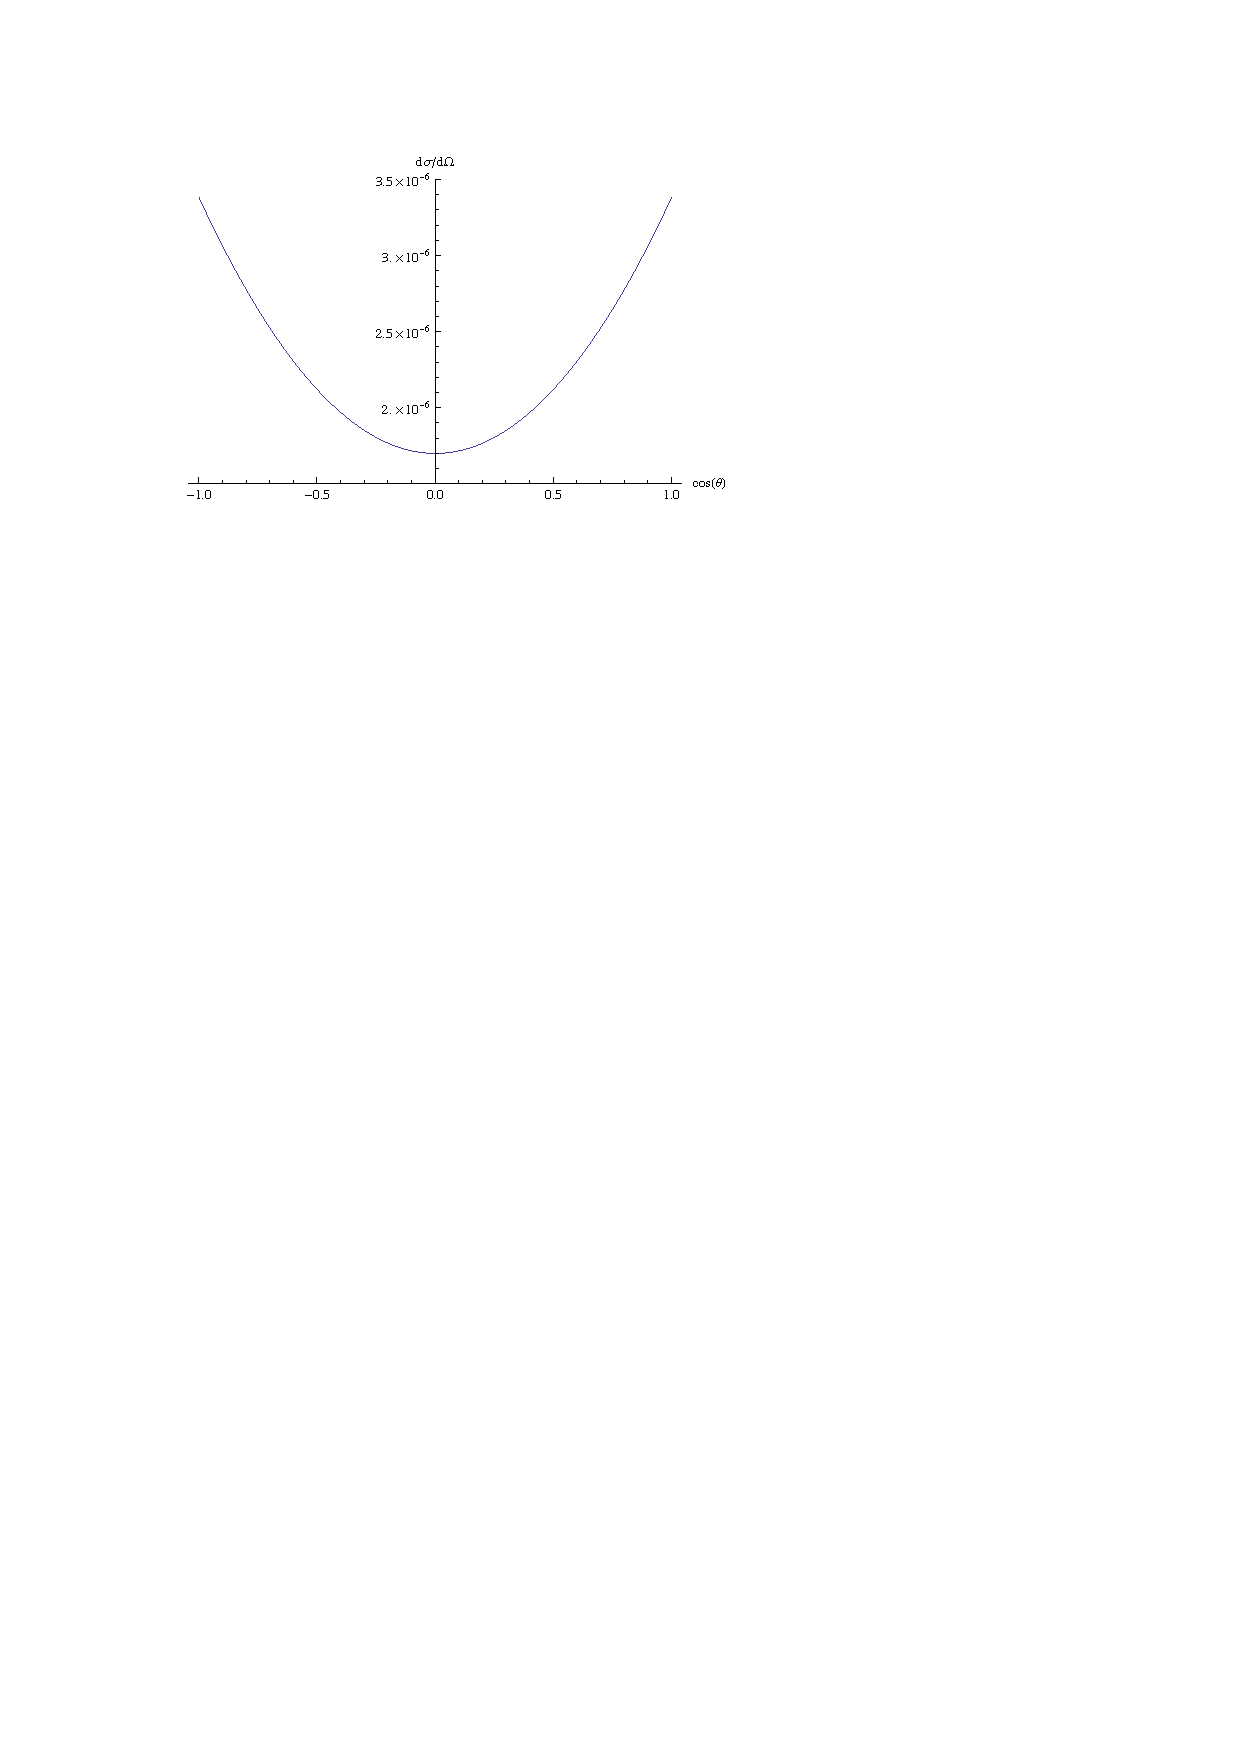
\includegraphics[scale=0.7]{sm_below}
	}
	\caption{$\frac{\d{\sigma}}{\d{\Omega}}$ at $\sqrt{s}=3\GeV$.}
	\label{fig:diffbelow}
\end{figure}

\begin{figure}[h]
	\vspace{10pt}
	\centering
	\subfloat[QED]{
		\label{fig:diffqedexact}
		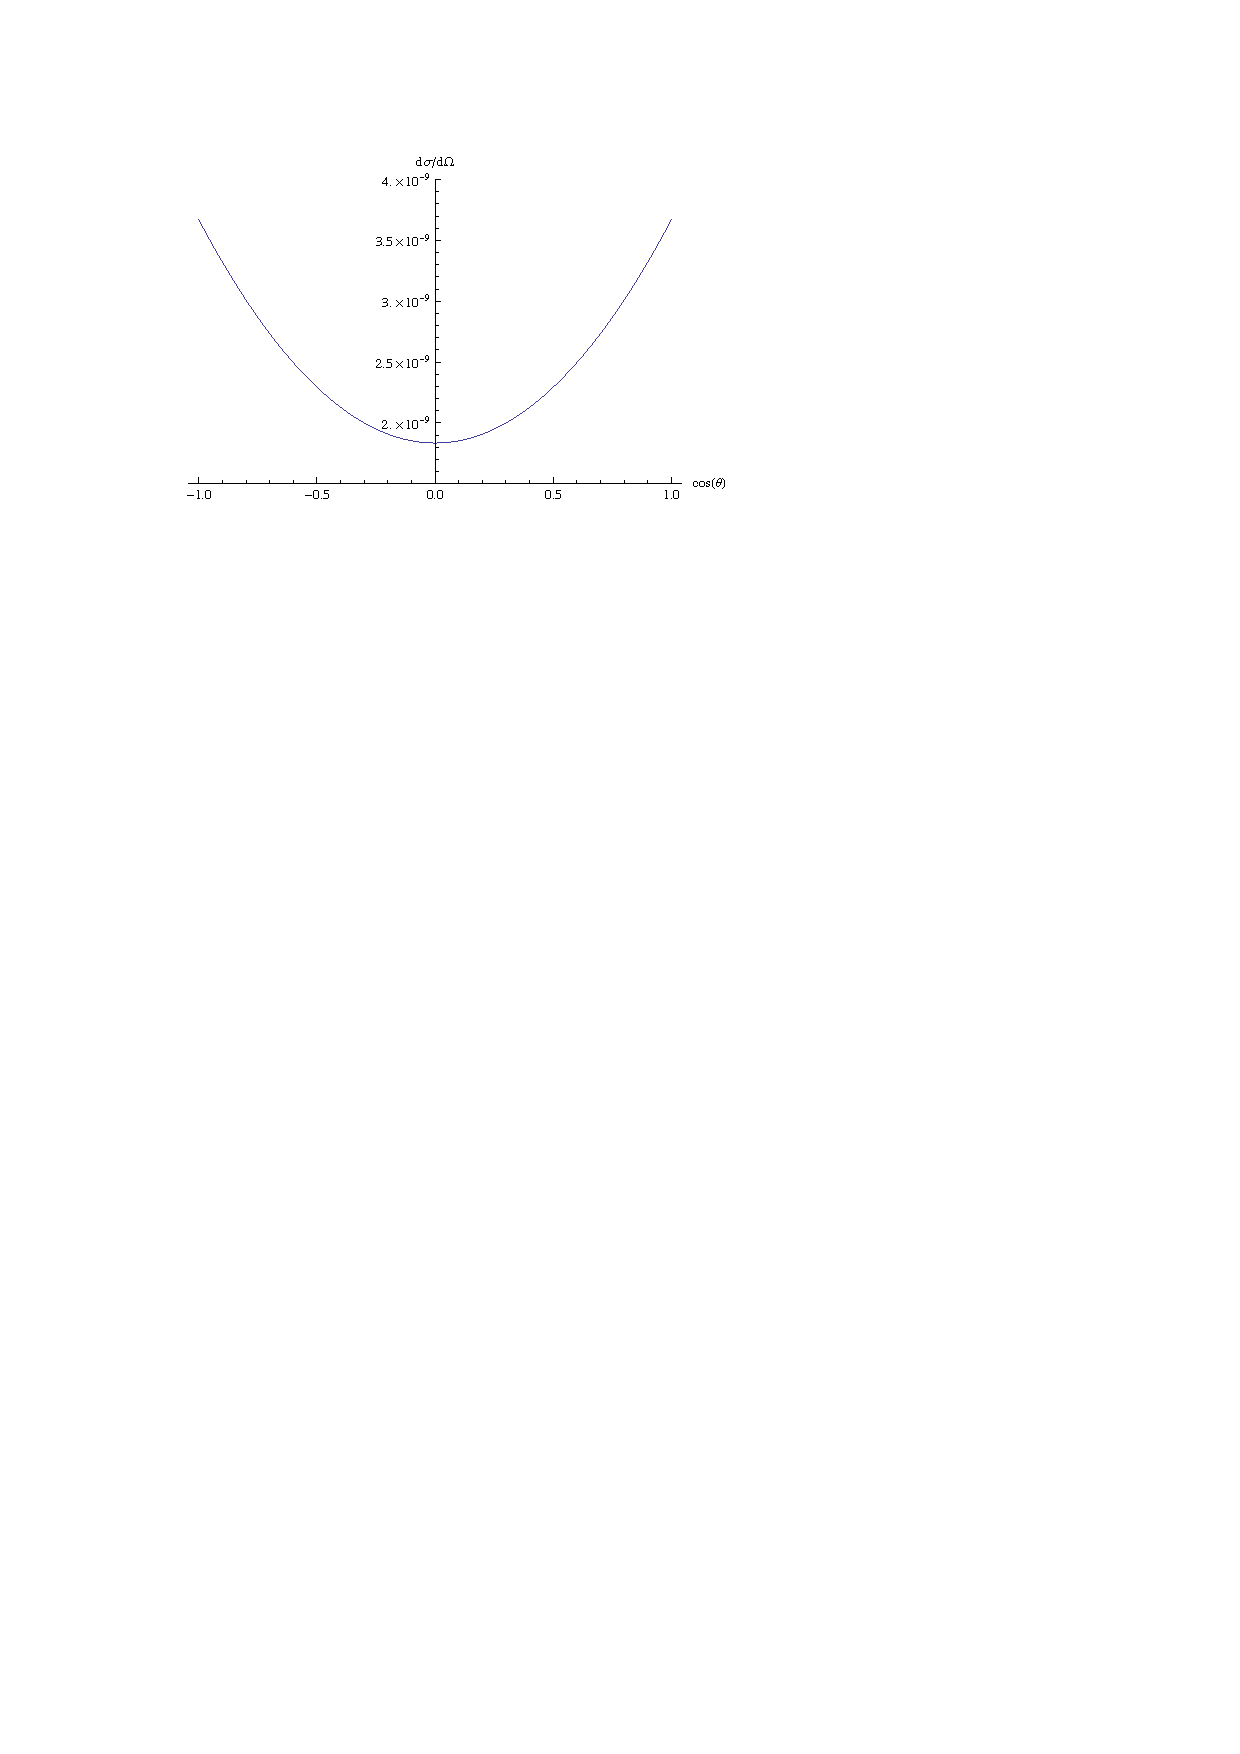
\includegraphics[scale=0.7]{qed_exact}
	}
	\subfloat[SM]{
		\label{fig:diffsmexact}
		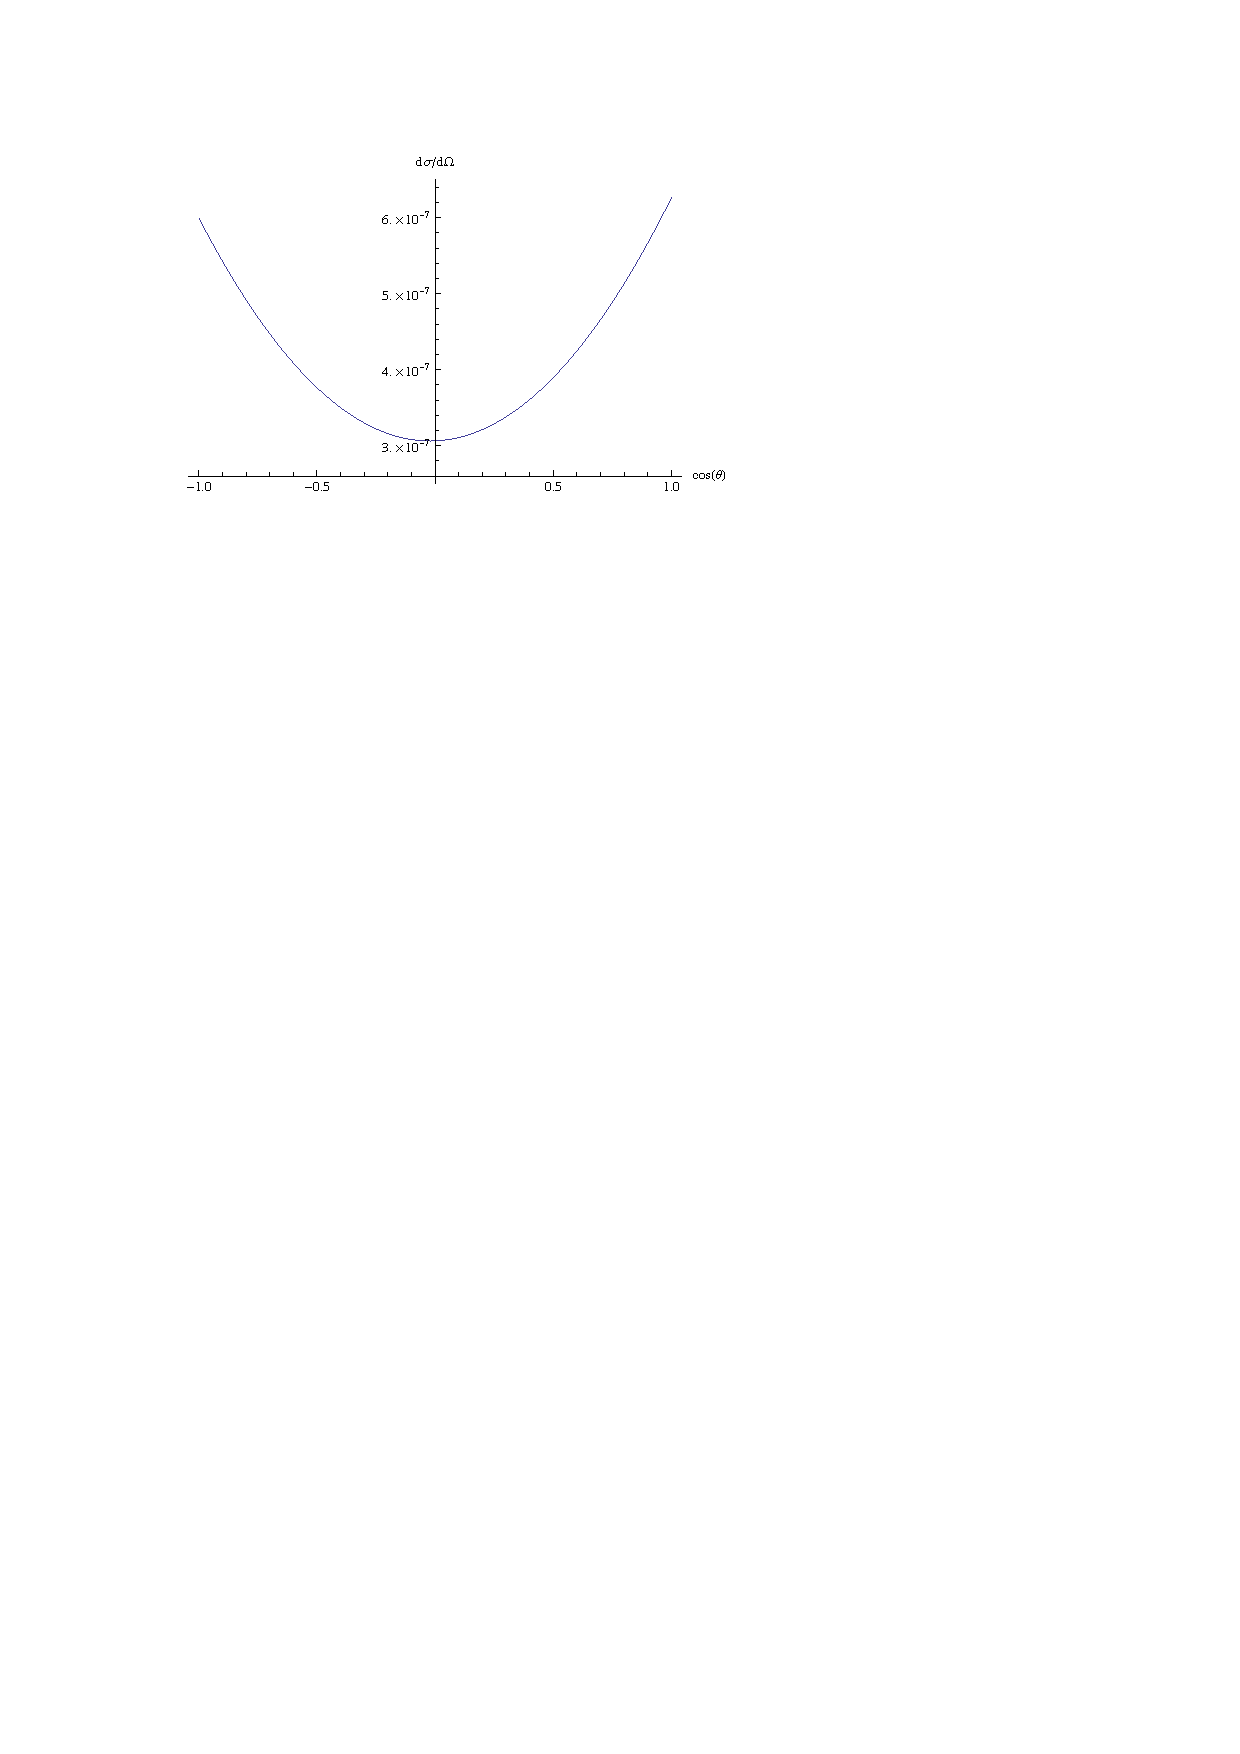
\includegraphics[scale=0.7]{sm_exact}
	}
	\caption{$\frac{\d{\sigma}}{\d{\Omega}}$ at $\sqrt{s}=M_{\Zzero}=91.2\GeV$.}
	\label{fig:diffexact}
\end{figure}

\begin{figure}[h]
	\vspace{10pt}
	\centering
	\subfloat[QED]{
		\label{fig:diffqedabove}
		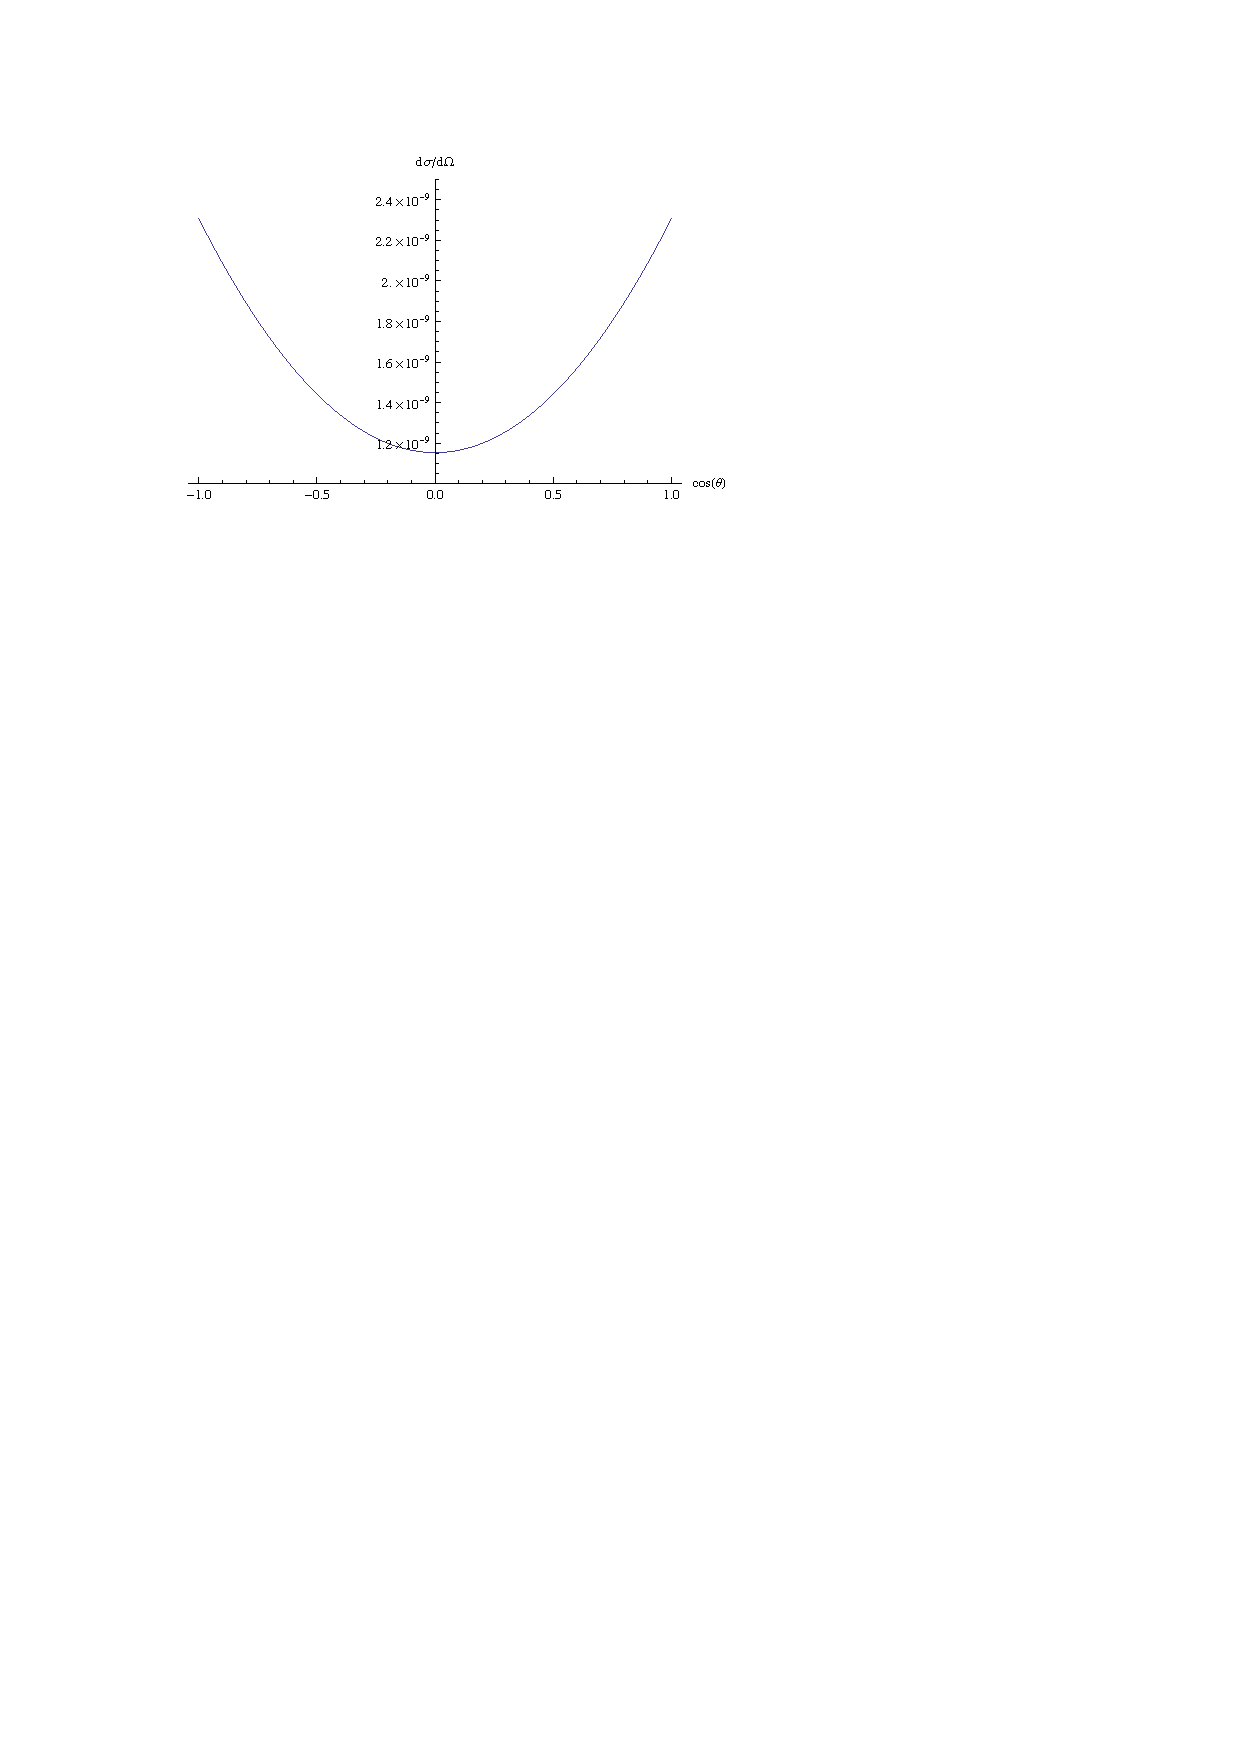
\includegraphics[scale=0.7]{qed_above}
	}
	\subfloat[SM]{
		\label{fig:diffsmabove}
		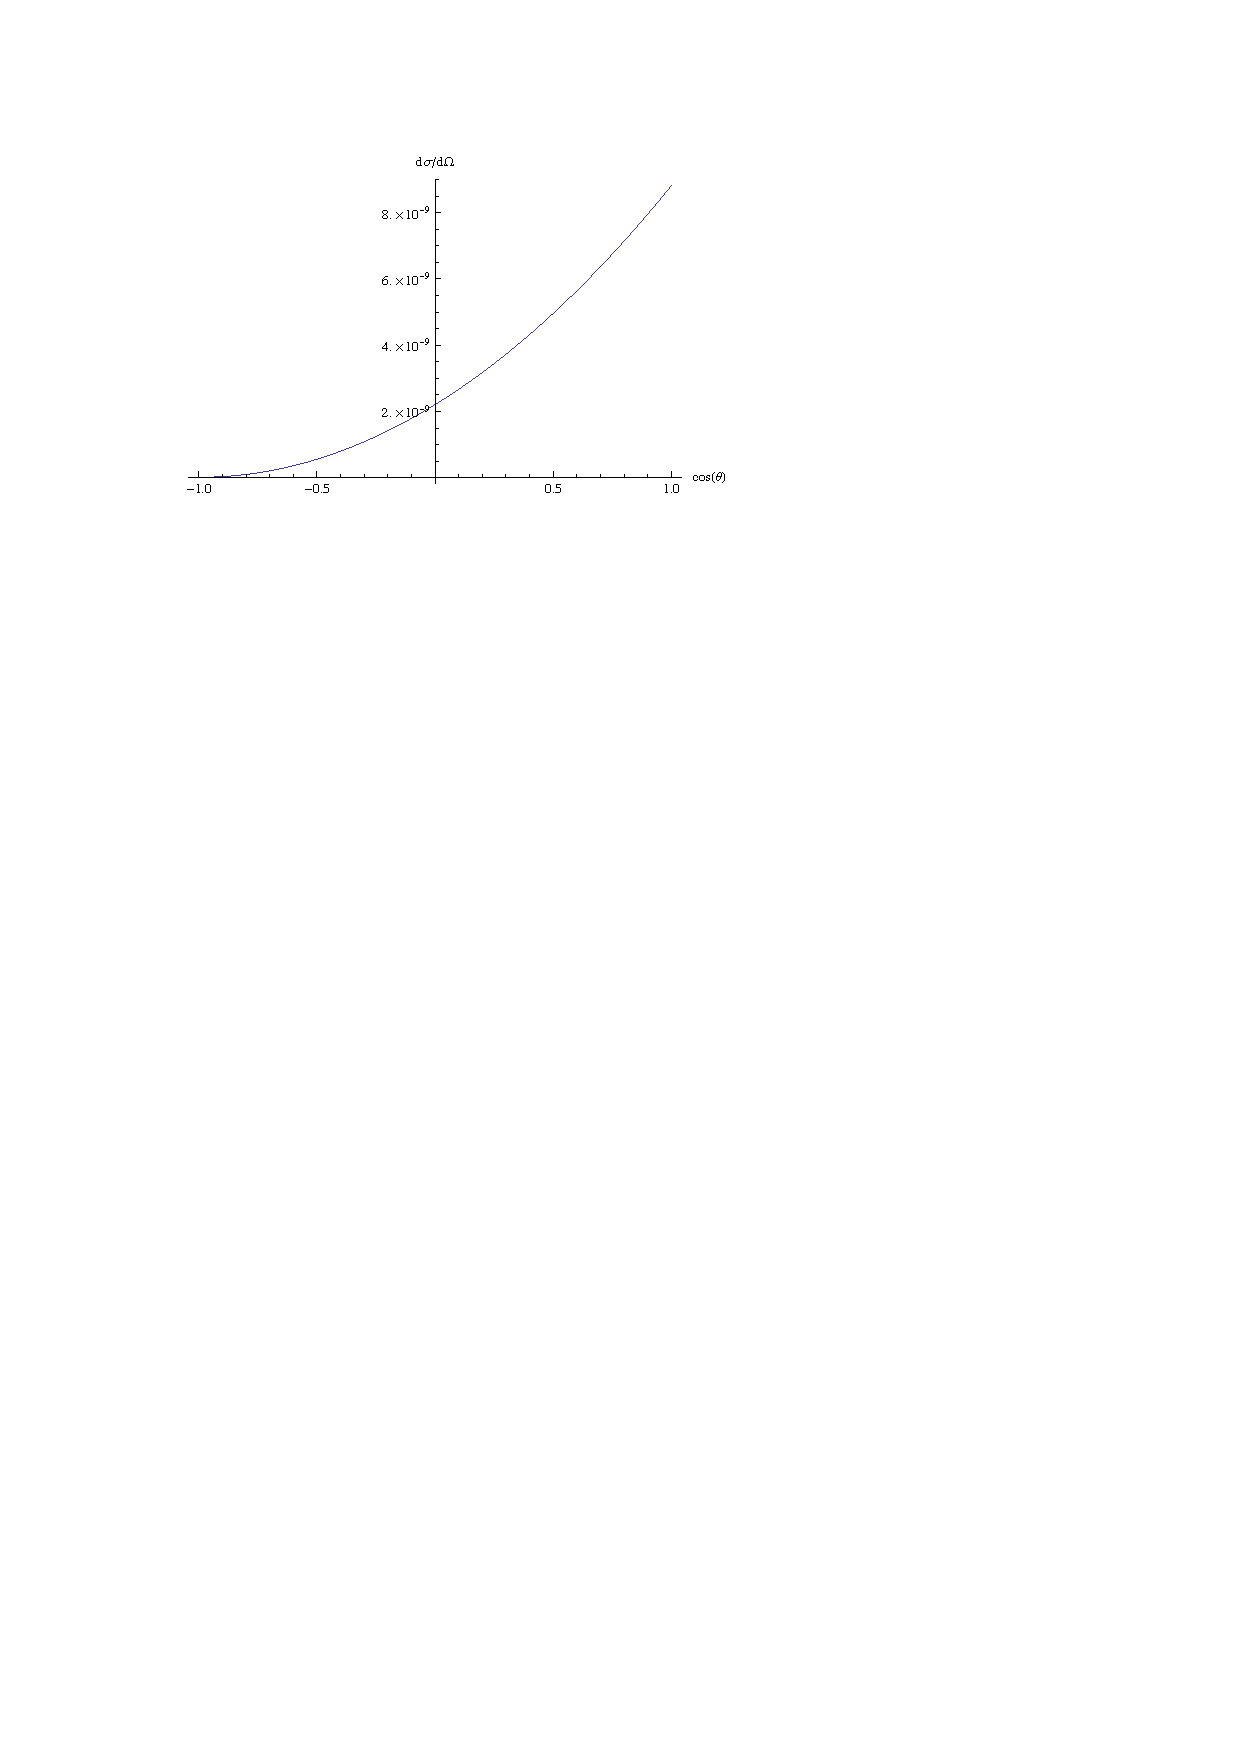
\includegraphics[scale=0.7]{sm_above}
	}
	\caption{$\frac{\d{\sigma}}{\d{\Omega}}$ at $\sqrt{s}=115\GeV$.}
	\label{fig:diffabove}
\end{figure}

\newpage

\appendix
\section{Differential Cross Sections}\label{app:differentials}

The cross sections corresponding to the photon, $\Zzero$ and interference matrix elements follow. Due to the length of the analytic solutions, constants are defined, then the cross section is defined with respect to these constants.

Due to the small energy scales that will be probed reachable at LEP, we consider the electromagnetic and weak coupling constants, $\alpha$ and $\theta_{w}$ respectively, as constant.\footnote{$\alpha$ is taken to be $\frac{1}{128}$, $\sin{\theta_{w}}^{2}$ is taken to be $0.23152$.}

\subsection{$\gamma\operatorname{-}\gamma$}

Define

$$
\alpha = \frac{g_{e}^{4}}{(8\pi)^{2}s} \sqrt{1-4\varepsilon^{2}}.
$$

Then

$$
\frac{\d{\sigma}}{\d{\Omega}}^{\gamma\operatorname{-}\gamma} = \alpha (1 + \cos^{2}{\vartheta} + 4\varepsilon^{2}\sin^{2}{\vartheta}),
$$
\begin{equation}
\sigma^{\gamma\operatorname{-}\gamma} = \frac{16\pi\alpha}{3}(1 + 2\varepsilon^{2}).
\end{equation}

\subsection{$\Zzero\operatorname{-}\Zzero$}

Define

\begin{align*}
\alpha &= \frac{g_{\Zzero}^{4}}{(32\pi)^{2}s} \frac{\sqrt{1-4\varepsilon^{2}}}{(1-\lambda^{2})^{2} + (\frac{\lambda\GZ}{\rts})},
\\
\beta &= ((C_{V}^{e})^{2} + (C_{A}^{e})^{2})((C_{V}^{\mu})^{2}),
\\
\Gamma &= ((C_{V}^{e})^{2} + (C_{A}^{e})^{2})((C_{A}^{\mu})^{2})(1-4\varepsilon^{2}),
\\
\Delta &= 8C_{V}^{e}C_{A}^{e}C_{V}^{\mu}C_{A}^{\mu}\sqrt{1-4\varepsilon^{2}}.
\end{align*}

Then

$$
\frac{\d{\sigma}}{\d{\Omega}}^{\Zzero-\Zzero}
  = \alpha(\beta(1+\cos^{2}{\vartheta}+4\varepsilon^{2}\sin^{2}{\vartheta})
    + \Delta(1+\cos^{2}{\vartheta})
    + \Gamma\cos{\vartheta}
  ),
$$
\begin{equation}
\sigma^{\gamma\operatorname{-}\gamma} = \frac{16\pi\alpha}{3}(\Gamma + (1 + 2\varepsilon^{2})\beta).
\end{equation}

\subsection{$\gamma\operatorname{-}\Zzero$}

Define

\begin{align*}
\alpha &= \frac{g_{\Zzero}^{4}}{(32\pi)^{2}s} \frac{\sqrt{1-4\varepsilon^{2}}}{(1-\lambda^{2})^{2} + (\frac{\lambda\GZ}{\rts})},
\\
\beta &= ((C_{V}^{e})^{2} + (C_{A}^{e})^{2})((C_{V}^{\mu})^{2}),
\\
\Gamma &= ((C_{V}^{e})^{2} + (C_{A}^{e})^{2})((C_{A}^{\mu})^{2})(1-4\varepsilon^{2}),
\\
\Delta &= 8C_{V}^{e}C_{A}^{e}C_{V}^{\mu}C_{A}^{\mu}\sqrt{1-4\varepsilon^{2}}.
\end{align*}

Then

$$
\frac{\d{\sigma}}{\d{\Omega}}^{\gamma-\Zzero}
  = \alpha(\beta(1+\cos^{2}{\vartheta}+4\varepsilon^{2}\sin^{2}{\vartheta})
    + \Delta\cos{\vartheta}
  ),
$$
\begin{equation}
\sigma^{\gamma-\Zzero} = \frac{16\pi\alpha\beta}{3}(1 + 2\varepsilon^{2}).
\end{equation}

\begin{thebibliography}{9}
  % type bibliography here
\end{thebibliography}

\end{document}